\section*{Stichpunkte%
         \label{sec:}}
         
imu (inertia measurement unit):
innere Korrektur-Werte eingestellt (Automatisch Anfang und manuell nachjustiert)
Ziel war es, den Betragsvektor in jeder Orientierung, auf die Größe der Gravitationsbeschleunigung zu bekommen. 

Gesamtziel: Längs und Querdynamic steuerung und regelung. Einschließlich schlupfregelung QUATSCH!!!!

Was bisher geschah:

-Skript geschrieben um den Laptop mit dem Jetson des Autos zu verbinden. (ROS-Master/Slave System)\\
Das dient vor allem dazu, das ich die Skripte auf meinem Laptop ausführen kann was mir schnelleres Arbeiten und das schnelle starten von Tests.

-Skript geschrieben um das Fahrzeug linear zu bewegen. (\lstinline{move_base.py})\\
Dieses Skript wartet auf ein Signal das entweder 0 ist um zu stoppen oder 1 um nach vorne zu fahren in einer bestimmten Geschwindigkeit (Diese ist fix und kann nicht vom Signal übergeben werden). Damit können umfangreiche Tests bezüglich der Beschleunigungs- und Geschwindigkeitsmessung gemacht werden.

-Ein Skript wurde erstellt um die Beschleunigung des resultierenden Vektors zu messen (\lstinline{imuorientation.py})\\
Dieses Skript dient dazu diverse Tests mit der IMU durch zu führen. Durch umfangreiche Versuche wurden so Ungereimtheiten mit der Kalibrierung behoben (Oder eher Verbessert). Hier wird das Topic der IMU abgefangen und einige Zyklen ein Durchschnittswert bestimmt. Der Durchschnittswert soll verhindern das Ausreißer zu viel Einfluss nehmen auf die Tests.

-Zwei Skripte geschrieben um diverse Tests mit der IMU und der Odometrie durch zu führen

    -Einmal wurde das Signal der IMU Integriert um aus der Beschleunigung eine Geschwindigkeit zu bekommen (Hier muss natürlich deutlich mehr Inhalt und Referenzen rein.)
    
    -Zum Schluss wurde das Signal der Odometrie Differenziert um aus der Geschwindigkeit der Odometrie eine Beschleunigung zu bekommen. (Das war analog zum anderen und hat deutlich weniger Aufwand gekostet, könnte natürlich aber auch weiter ausgeführt werden)
    
Zudem musste die IMU Kalibriert werden. Ursprünglich hat die IMU sich mit jedem Neustart selbst Kalibriert, das führte dazu das teilweise die Werte nicht das bestmögliche Resultat lieferten, weshalb wir die IMU getestet haben und die Werte Manuell angepasst haben. (Dieser Vorgang ist noch nicht ganz abgeschlossen da das Ergebnis noch immer nicht ganz Zufriedenstellend ist). 
Das ganze ist notwendig damit die Erdbeschleunigung anschließend sauber raus gerechnet werden kann. Da die IMU sich neigen kann während der Fahrt oder sogar uneben Montiert ist, muss die Erdbeschleunigung raus gerechnet werden um den Drift während des Messens zu minimieren.
Die IMU wurde zudem Software-seitig gedreht mit dem IMU transformer Skript.

Notizen zum 20.04:

IMU Orientierung mit Quaternionen verrechnen um die Erdbeschleunigung zu bekommen. Hierzu wurde das Skript \textbf{imuorientation.py} kopiert und in \textbf{imutests} erweitert um Quaternionen Multiplikation und das bestimmen des Konjugierten Quaternion.
Besonders Hilfreich war dieser \href{https://stackoverflow.com/questions/60492369/gravity-compensation-in-imu-data}{\emph{\textbf{Thread}}}

Die IMU daten werden mit dieser \href{https://docs.ros.org/en/noetic/api/sensor_msgs/html/msg/Imu.html}{\emph{\textbf{Massage}}} Syntax versendet

Mit der Multiplikation von der Ausrichtung als Quaternionen und dem Beschleunigungsvektor kann man die Ausrichtung auf das Erdkoordinatensystem transformieren. Danach ist es möglich den Vektor [0, 0, 9.81] ab zu ziehen und man erhält einen stets bereinigten Sensorwert.

In einem kleinen Test habe ich das ausführlich getestet. Dabei ist raus gekommen das sich der Sensor mittlerweile bis auf zwei Nachkommastellen genau verhält.
Die Werte stehend auf den Rädern auf 4 Nachkommastellen gekürzt.

acc mean: -0.0268 0.0724 -0.0567

roll mean: 1.3763 pitch mean -0.3406 yaw mean: -0.0638

Betrag: 0.0958

Der Betrag weicht immer noch fast ein Zehntel von 0 ab. Das hängt damit zusammen das die Kalibrierung des Sensors noch Abweichungen zu lässt.

Probleme: \\
Es ist derzeit noch ein Problem das nicht der schon bereits gedrehte IMU-Frame genutzt werden kann. Da die Orientierung in diesem nicht geändert wird! Die Frage ist hier ob wir einfach mit dem auf das Erdkoordinaten ausgerichtete System weiter arbeiten können. prinzipiell wäre hier X immer die lineare Bewegung und immer die Querkräfte. 

Weitere nützliche Links:\\
\href{https://stackoverflow.com/questions/39000758/how-to-multiply-two-quaternions-by-python-or-numpy}{\emph{\textbf{Quaternionen Multiplikation in Numpy}}}

Notizen vom 23.04:
\lstinline{imu_gravity_remover} geschrieben. Dieses Script nimmt die daten der IMU und rechnet die Erdbeschleunigung raus. Dieses Skript sendet dann die Daten weiter.
geplant ist das Skript noch in ein cpp skript zu schreiben.

\begin{figure}[H]
  \begin{center}
  
    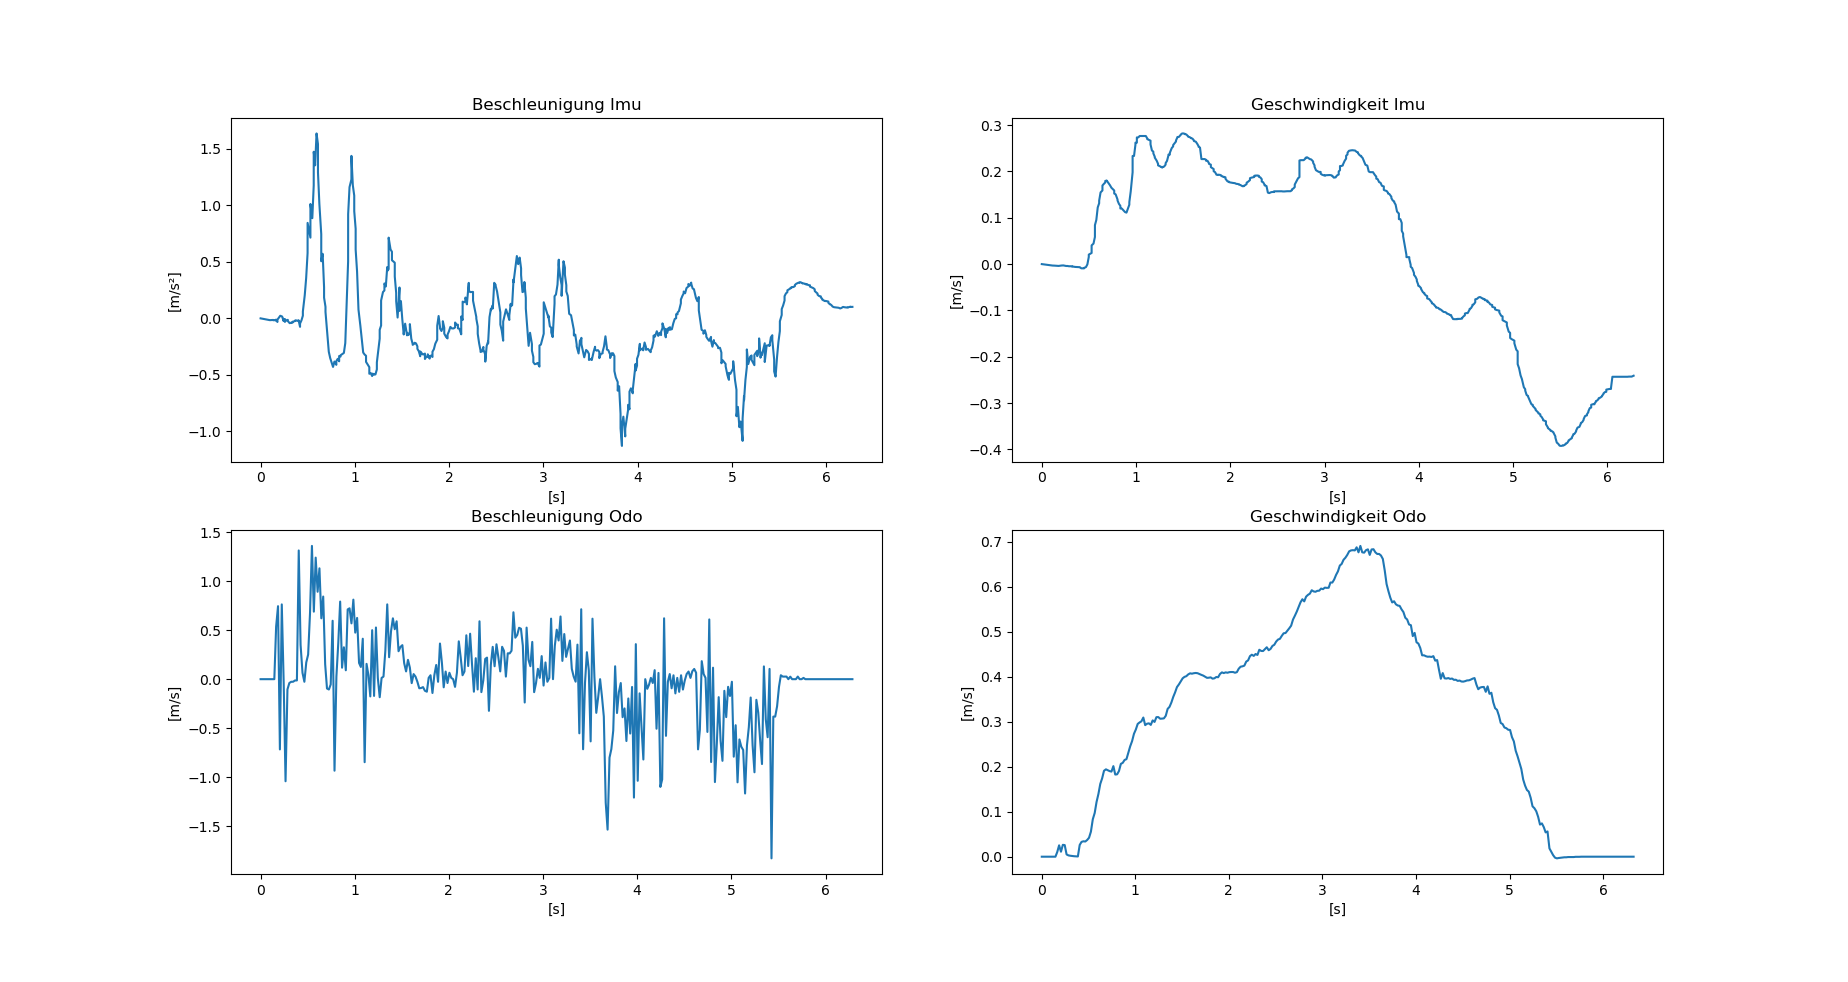
\includegraphics[width=\textwidth]{bilder/23AprImuOdoBeschlGeschw.png}
  \caption{Einzelne Diagramme der Beschleunigung sowie der Geschwindigkeiten}
  \label{fig:diagram1}
  
    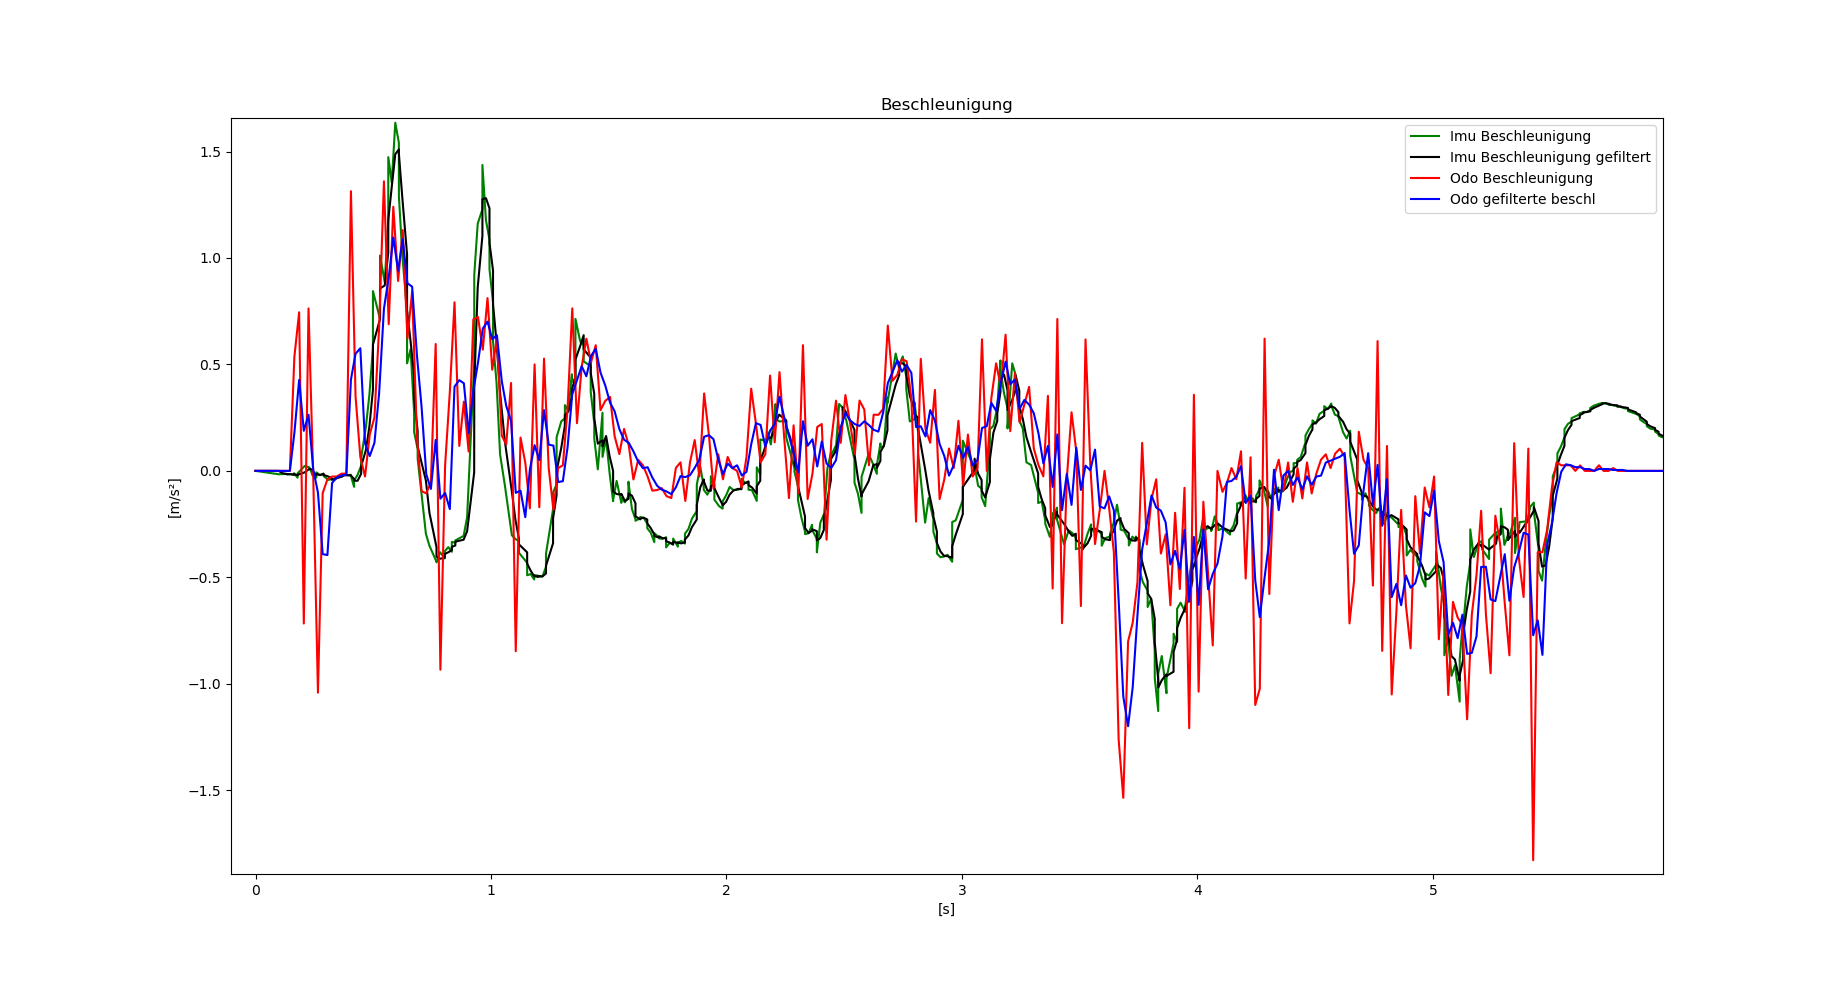
\includegraphics[width=\textwidth]{bilder/23AprBeschlOverlap.png}
  \end{center}
  \caption{Beschleunigungswerte übereinander gelegt aktueller Stand}
  \label{fig:diagram2}
\end{figure}

Wie hier im Bild zu sehen ist, ist das Differenzieren der Odometrie mit recht viel Rauschen verbunden. Im zweiten Diagramm sieht man auch das die Abtastrate sehr ungleichmäßig ist. Derzeit liegt die Vermutung nahe, dass die Skripte nicht schnell genug sind. 
Zudem ist der Drift des Imu immer noch sehr Stark. Die überlegung ist hier mit einem Filter zu arbeiten falls notwendig.

Notizen vom 27.04:
neue Funktion hinzugefügt im \lstinline{cmd_vel_switcher}, um einen Halbautomatischen Modus zu realisieren. Dazu wurden zwei Topics miteinander vermischt und das Signal wieder auf gepublished.

    sec: 1672855594
    nanosec: 699926525
    sec: 1672855594
    nanosec: 715770401
    sec: 1672855594
    nanosec: 731787777
    sec: 1672855594
    nanosec: 731886526
    sec: 1672855594
    nanosec: 747749124
    sec: 1672855594
    nanosec: 764142540
    sec: 1672855594
    nanosec: 764315234
    sec: 1672855594
    nanosec: 779952251


Ausblick dem Arduino das beibringen die Zeit mit zu senden.


